%% Standalone supplementary material: FEniCSx cross-code consistency check of collapsibleChannel.
%% DRAFT. Build (from this directory):  latexmk -pdf supplement_fenicsx_collapsiblechannel.tex
%% It does not read article.aux (no cross-references to the main article), so it builds on its own.
%% Bibliography key Baratta2023 (DOLFINx) is added to bibliography.bib byte-identically by the open draft PRs #69 and #70 and by this branch; PETSc, MUMPS:1, MUMPS:2, are already in bibliography.bib.
%% Data, scripts, provenance, preflight, hypothesis bookkeeping, formulation controls and deviations: paper-data/fenicsx_collapsiblechannel/ (README.md there).
\documentclass[sn-mathphys,Numbered]{sn-jnl}
\usepackage{graphicx}
\usepackage{amsmath,amssymb,amsfonts,bm}
\usepackage{xcolor}
\usepackage{soul}
\usepackage{manyfoot}
\usepackage{booktabs}
\usepackage{siunitx}
\usepackage{float}
\usepackage[utf8]{inputenc}
\usepackage[onehalfspacing]{setspace}
\usepackage{placeins}
\usepackage{geometry}
\geometry{a4paper,textwidth=15cm,textheight=24cm}
\setlength{\parskip}{0.5\baselineskip}
\raggedbottom

%% S-prefixed numbering
\renewcommand{\thesection}{S\arabic{section}}
\renewcommand{\thefigure}{S\arabic{figure}}
\renewcommand{\thetable}{S\arabic{table}}
\renewcommand{\theequation}{S\arabic{equation}}

\newcommand{\todo}[1]{\par\noindent\textcolor{red}{\rule{\linewidth}{0.8pt}}\par\nopagebreak
	\noindent{\small\color{red!70!black}\textbf{AUTHOR NOTE:} #1\par}\nopagebreak
	\noindent\textcolor{red}{\rule{\linewidth}{0.8pt}}\par}
%% Qualifier carried by every agreement statement against the extrapolated oomph-lib solution.
\newcommand{\urefFull}{{\small[oomph reference: first-order extrapolation, not an uncertainty bound (\ref{sec:cc_model}), same group; model form unresolved]}}
\newcommand{\urefOne}{{\small[oomph refine-1 reference: spatial error $0.19\,\%\,P$ at the trough, same group; model form unresolved]}}
\newcommand{\uref}{{\small[qualifiers as in \ref{sec:cc_offset}]}}
\newcommand{\legbc}{\textcolor{red!70!black}{(legacy, pre-\#671)}}
\newcommand{\pP}{\ensuremath{\,\%\,P}}
\makeatletter
\renewcommand{\paragraph}[1]{\par\vspace{0.3\baselineskip}\noindent\textbf{#1}\ }
\makeatother

\begin{document}

\title[Supplementary material: FEniCSx collapsibleChannel]{Supplementary material: a same-lineage cross-code check of collapsibleChannel with a monolithic FEniCSx implementation}

\author*[1]{\fnm{Author} \sur{Placeholder}}\email{corresponding.author@example.org}
\author[1]{\fnm{Author} \sur{Placeholder 2}}

\affil[1]{\orgdiv{School of Mechanical and Materials Engineering}, \orgname{University College Dublin}, \orgaddress{\country{Ireland}}}

\maketitle

\todo{DRAFT, supplementary to the collapsibleChannel material (PRs \#30, \#45, \#51, \#74). Author list, CRediT and the AI-use paragraph are placeholders for the authors to agree. Numbers come from the CSV files in \texttt{paper-data/fenicsx\_collapsiblechannel/}; provenance, preflight results, hypothesis bookkeeping, formulation controls, deviations and the retained failed runs are in its README. \textbf{The solver repository is private and the raw run output is not yet public}; the tables here cannot be reproduced from this PR alone until an archived snapshot exists (needed before submission). No manuscript text and no classification (category~B) is changed.}

\section{Scope and disclosure}\label{sec:cc_scope}
This supplement is a \emph{same-lineage cross-code check} of the collapsibleChannel tutorial: a monolithic ALE finite-element implementation (FEniCSx) on three spatial levels and four time steps, compared at equal time step with the oomph-lib solution and with the solids4foam mesh study. It is \textbf{not an independent validation}. The code, preregistration, runs, analysis and one internal audit (QUALIFIED; not a human or external review) were produced by AI agents of one model family for the same group that produced the solids4foam and oomph-lib reference runs; definitions, normalisation and monitoring points are shared, so a shared misreading would be invisible. No external review has taken place. ``Preregistered'' means written before the runs, with self-asserted timestamps.
\paragraph{Registered outcomes and status of the findings.}
Registered: H1 (spatial) falsified; H2 (time) passes three rows and fails the last as written (marginal); H2x (separability) additive but vacuous; H3 (agreement with a spatial limit) not evaluable; H4a, H4c, H5, H7, H8 pass; H4b untested; preflight criteria missed or failed are listed in the README. \textbf{Not preregistered} (exploratory): the successive-difference comparison with oomph-lib, the offset analysis, the comparison with the extrapolated oomph-lib solution (published by the authors of the tutorial after our runs), the error correlation and the window statistics; the open-loop replay (MF1) was preregistered after the production results and the offset were known. After excluding these, what survives as registered is: the solver runs and its gates pass, H1 failed, H2 is marginal. We give no spatial order and no spatial limit of our own.

\section{Model, solver, runs and references}\label{sec:cc_model}
\paragraph{Problem.}
A channel $[0,25]\times[0,1]$ with a collapsible wall on $5\le x\le15$ (thickness $0.05$, plane-strain St~Venant--Kirchhoff, $E=4.55\times10^{8}$, $\nu=0.3$, $\rho_s=1$, clamped end faces), fluid $\rho_f=1$, kinematic viscosity $0.02$; total-traction ends $p_\mathrm{in}=6$, $p_\mathrm{out}=0$, external follower pressure ramped as $200\,(1-\cos(\pi t/0.25))/2$ and held at $200$ afterwards, Poiseuille start, $1.5\,\mathrm s$. The tutorial's ends are fixed pressure with zero-gradient $u_x$; the FE primary uses natural total traction with $u_y$ strong (the tutorial form, FM5, changes the first trough by $\le1.4\times10^{-5}\,\%\,P$). Values are percent of the nominal peak $P=0.216\,\mathrm m$ (the peak of the refine-1 reference, a constant) at $x=7.5,10,12.5$. The FE values are on the fluid-facing (bottom) face, the headline comparison although the oomph wall is a beam axis (the midplane is the like-for-like face; the bottom face is the conservative choice).
\paragraph{Solver and runs.}
DOLFINx~\citep{Baratta2023}, PETSc SNES~\citep{PETSc}, MUMPS~\citep{MUMPS:1,MUMPS:2}; one monolithic system $(\bm u\,P_2,\ p\,P_1,\ \bm d\,P_2)$ on one triangle mesh, a total-Lagrangian continuum wall with shear and rotary inertia, exact Nanson traction; the interface and ALE velocities are the same BDF2 derivative of the displacement (backward Euler on step~1) and the wall inertia applies BDF2 once more, the solids4foam \texttt{backward} operator. Meshes S1, S2, S3: fluid $25n_y\times n_y$ squares split into triangles, $n_y=8,16,32$, wall $10n_y\times4$ conforming elements (the wall resolution is \emph{tied} to the fluid mesh); $\Delta t=0.025$ (S1, S2), $0.0125$, $0.00625$, $0.003125\,\mathrm s$ (S3 at $0.003125$ ends at $1.25\,\mathrm s$). 26 production jobs (25 cells, one cancelled), 11.03 CPU-h; all cells converged. The first trough $V_1$ is found on a cubic Hermite interpolant through the stored displacement and BDF2 interface velocity (first trough in $0.3\le t\le0.75\,\mathrm s$; oomph-lib by cubic spline; effect $\le0.003\,\%\,P$); the FE value is on the fluid-facing (bottom) face, the midplane is deeper by $0.007\,\%\,P$ at $x=10$ and $0.021$--$0.025$ at the quarter points.
\paragraph{References.}
(i) The tutorial's oomph-lib reference is a regenerated oomph-lib solution (Kirchhoff--Love beam, $E_\mathrm{eff}=E/(1-\nu^2)$, translational inertia, regularising wall density; no pre-stress, clamped, ramped pressure; Richardson in time) of the tutorial's modified problem, produced by the same group, at the tutorial resolution (refine~1). The same-$\Delta t$ runs ($\Delta t=0.025$ to $0.003125$) are also refine~1. (ii) The authors' refinement study (PR~\#74, refine 1 to 4 at $\Delta t=0.00625$) shows that oomph-lib converges at \emph{first order} in space and that refine~1 has a spatial error of $0.53\,\%$ of the peak in the mid-wall history (L$_\infty$; $0.38$, $0.37$ at the quarter points; first trough $+0.19$ at $x=10$, $+0.13$ at the quarter points); the earlier estimate of $0.26\,\%\,P$ (refine~1 against 2 at $\Delta t=0.025$) is superseded. The solution extrapolated to zero mesh size (first order from refine 3 and 4; the $(2,3)$ extrapolation agrees with it to $0.004\,\%\,P$, which only checks two $p=1$ extrapolations of the same runs against each other and is \emph{not} an uncertainty bound: assuming order $1.25$ would move the first trough by up to $0.011$ and the history by up to $0.028\,\%\,P$, order $1.5$ by $0.018$ and $0.046$, the size of the residual offsets below; \texttt{data/extrapolation\_order\_sensitivity.csv}) exists \textbf{only at $\Delta t=0.00625$}; its first trough is $-68.760$, $-100.068$, $-69.975\pP$ at $x=7.5,10,12.5$. All comparisons with it are at $\Delta t=0.00625$ only; extrapolated references at other $\Delta t$ were not available. (iii) solids4foam F1--F4 (PR~\#51): Robin--Neumann, $\Delta t=0.00625\,\mathrm s$, build a421f063d, MeluXina, 2 Nov 2026, \textbf{before} solids4foam PR~\#671 (legacy wall BC; the \#671 effect on this tutorial is bounded at $\le0.09\,\%$ ($0.074$, $0.078$, $0.086$ at the three points, each normalised by its own maximum) for IQN-ILS at $\Delta t=0.025$ only, and was not A/B tested for the Robin, $\Delta t=0.00625$ baseline over the full run (only a start-up window $t\le0.325\,\mathrm s$, ending before the first trough, showed $0.0011\,\%$); reported by the \#671 study, not recomputed).

\section{Time behaviour at equal time step}\label{sec:cc_time}
The change of the first trough between successive time steps needs no limit and, if the reference's spatial error does not change with $\Delta t$, cancels it (Table~\ref{tab:cc_succ}; \texttt{data/successive\_trough\_differences.csv}). At $x=10$ the S2 sequence agrees with the refine-1 oomph-lib same-$\Delta t$ sequence to $0.014$, $0.006$, $0.003\,\%\,P$ (over all positions and meshes the mismatch is up to $0.026$; \texttt{data/successive\_difference\_mismatch\_range.csv}) \urefOne{} (refine-1 spatial error $0.19\,\%\,P$ at the trough, assumed constant in $\Delta t$, not tested: the extrapolated solution exists at one $\Delta t$ only, so the table could not be redone).
\begin{table}[!htb]
\centering
\caption{Change of the first trough at $x=10$ between successive $\Delta t$ (\pP); oomph-lib: tutorial resolution (refine 1), same $\Delta t$.}\label{tab:cc_succ}
\small
\begin{tabular}{@{}lrrrrr@{}}
\toprule
$\Delta t$ (s) & FE S1 & FE S2 & FE S3 & oomph-lib & S2 minus oomph \\
\midrule
$0.025\to0.0125$ & $-1.045$ & $-1.037$ & -- & $-1.023$ & $-0.014$ \\
$0.0125\to0.00625$ & $-0.248$ & $-0.247$ & $-0.246$ & $-0.253$ & $+0.006$ \\
$0.00625\to0.003125$ & $-0.106$ & $-0.101$ & $-0.100$ & $-0.104$ & $+0.003$ \\
\bottomrule
\end{tabular}
\end{table}
The pattern is not second order throughout (orders about $2.1$ then $1.3$ of the first trough in $\Delta t$, not the history orders of the main text). Hypothesis H2, built on the deficits against the FE time limit, passes at the first three rows at the observed order and is marginal at the last (row-by-row table and limit band in the README); the successive differences, not the deficit test, are the evidence here.

\section{First trough: offset to oomph-lib and model form}\label{sec:cc_offset}
\paragraph{Against the refine-1 reference (historical).}
At the same $\Delta t$ the FE trough at $x=10$ is deeper than the refine-1 oomph-lib trough by $0.147$ to $0.161\,\%\,P$ (S2) and $0.169$ to $0.179$ (S3), \emph{constant} in $\Delta t=0.025\to0.003125$ (at the quarter points $0.05$ to $0.11$). A constant offset is what a $\Delta t$-independent error of the reference produces, and it is not temporal truncation.
\paragraph{Against the extrapolated reference (this supplement's comparison).}
At $\Delta t=0.00625$ the offset changes size and sign (Table~\ref{tab:cc_off}; Fig.~\ref{fig:cc_time}). The refine-1 reference is shallower than the extrapolated one by $0.19$ ($x=10$) and $0.13\,\%\,P$ (quarter points), which accounts for most of the old offset: for S3 at $x=10$, $0.0196-0.1925=-0.173$. The remaining difference is small and positive (the FE trough is \emph{shallower}): bottom face $+0.020$ (S3) to $+0.038$ (S2) at $x=10$ and $+0.033$ to $+0.061$ at the quarter points; midplane $+0.012$, $+0.030$ at $x=10$ (S3, S2) and $+0.010$ to $+0.038$ at the quarter points; S1 ($-0.002$ to $+0.066$) is not monotone with S2 and S3. The history difference to the extrapolated oomph (maximum over $t\le1.5\,\mathrm s$, bottom face, $\Delta t=0.00625$) is $0.075$ ($x=10$) and $0.065$, $0.069$ (quarter points) for S3, $0.095$--$0.105$ for S2 and $0.76$--$1.09$ for S1, against $0.57$ for S3 at $x=10$ with the refine-1 reference \urefFull{} (\texttt{data/history\_norms\_vs\_extrapolated\_oomph.csv}). The constant offset against the refine-1 reference was largely that reference's spatial error.
\begin{table}[!htb]
\centering
\caption{First-trough differences at $\Delta t=0.00625$ (\pP). Rows 1--2: the old and the new reference; rows 3--5: FE minus extrapolated oomph; row 6: open-loop continuum minus beam (MF1, S2 load). \texttt{data/offset\_to\_extrapolated\_oomph.csv}, \texttt{mf1\_vs\_extrapolated\_offset.csv}.}\label{tab:cc_off}
\small
\begin{tabular}{@{}lrrr@{}}
\toprule
 & $x=7.5$ & $x=10$ & $x=12.5$ \\
\midrule
FE S3 (bottom) minus refine-1 oomph & $-0.090$ & $-0.173$ & $-0.100$ \\
refine-1 oomph minus extrapolated & $+0.125$ & $+0.192$ & $+0.133$ \\
FE S3 (bottom) minus extrapolated & $+0.035$ & $+0.020$ & $+0.033$ \\
FE S3 (midplane) minus extrapolated & $+0.013$ & $+0.012$ & $+0.010$ \\
FE S2 (midplane) minus extrapolated & $+0.038$ & $+0.030$ & $+0.035$ \\
open-loop continuum minus beam (MF1) & $+0.053$ & $+0.033$ & $+0.056$ \\
\bottomrule
\end{tabular}
\end{table}
\begin{figure}[!htb]
\centering
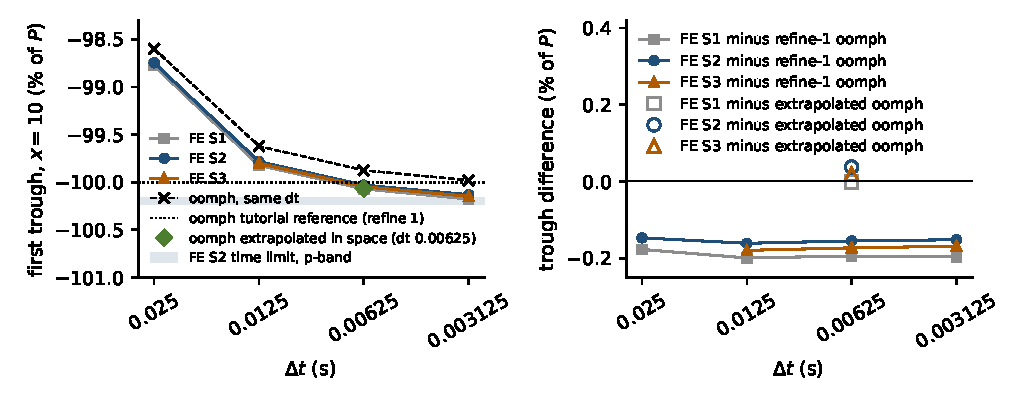
\includegraphics[width=0.6\textwidth]{paper-data/fenicsx_collapsiblechannel/figures/fenicsx_collapsible_trough_time}
\caption{Left: first trough at $x=10$ against $\Delta t$ for the three FE meshes, the refine-1 oomph-lib values, the refine-1 (time-extrapolated) reference, the extrapolated oomph value ($\Delta t=0.00625$) and the band of the S2 time limit. Right: FE minus refine-1 oomph at the same $\Delta t$ (constant) and FE minus extrapolated oomph at $\Delta t=0.00625$.}\label{fig:cc_time}
\end{figure}
\paragraph{Model form, re-evaluated (MF1).}
The open-loop replay applies the fluid load of one coupled run (S2, $\Delta t=0.00625$; normal and shear, stored every step) as a prescribed dead load to the continuum wall alone and to the oomph-equation beam (one element per $P_2$ wall element); its controls pass (rerun $1.7\times10^{-14}$, replayed continuum against the coupled wall $1.0\times10^{-7}$). The preregistered outcome (H6$'$: open-loop gap $\le0.15\,\%\,P$) is a pass: with 160 beam elements the signed trough difference continuum minus beam is $+0.053$, $+0.033$, $+0.056\,\%\,P$ (midplane; $0.040$--$0.078$ against the bottom face), i.e.\ the beam is deeper (Table~\ref{tab:cc_off}, row 6). The gap is resolved only marginally: with 80 beam elements the signed difference is $+0.021$, $-0.016$, $+0.022$, so at $x=10$ the \emph{sign flips} between 80 and 160 elements, the two beams differ by $0.033$--$0.049\,\%\,P$ (as large as the gap), and the registered resolution rule ($0.05$) is cleared at $x=10$ by $0.0008$ only; 320 elements were not run, so $0.033$--$0.056$ is not a bound. Against the \emph{old} reference the offset had the opposite sign; the earlier reading (``wrong sign to explain the offset'') is \textbf{withdrawn}. Against the extrapolated reference the midplane offset has the same sign as the 160-element gap and is smaller than it for S3 (the gap is $2.7$ to $5.7$ times the offset) and $0.6$ to $0.9$ of the gap for S2. This is consistent with the residual offset being model form, but not shown: the replay is open loop (dead load, one cell, load at the bottom face of the continuum and on the beam axis), the closed loop is not estimated, and the residual offset ($0.010$--$0.013$ for S3) is of the size of its other contributions: the FE spatial error (S2 against S3 changes the midplane offset by $0.018$--$0.025$), the extrapolation order (up to $0.011$ for order $1.25$), and the unresolved temporal mismatch at $\Delta t=0.00625$ between the FE and oomph time discretisations (successive-difference mismatch $0.003$--$0.006$ at $x=10$, $0.001$--$0.002$ at $x=12.5$, but $0.015$--$0.016$ at $x=7.5$, larger than the S3 residual offset there). Offsets of $0.010$--$0.013$ are therefore not resolved from the reference.

\section{Comparison with the solids4foam mesh study}\label{sec:cc_s4f}
All solids4foam values are the F1--F4 runs \legbc{} of PR~\#51 (wall midpoint). Against the extrapolated oomph the first-trough differences are $+0.227$, $+0.107$, $+0.046$, $+0.020\,\%\,P$ (F1--F4) and $+0.020$ for FE S3 at $x=10$; F4 and S3 differ by $-0.001\,\%\,P$ \uref. The history differences to the extrapolated oomph at $x=10$ ($L_\infty$, $t\le1.25$ / $1.5\,\mathrm s$) are $0.22$ / $0.33$ for F4 and $0.075$ / $0.075$ for FE S3 \uref; FE S3 minus F4 is $0.28$ / $0.40$ (S2: $0.30$ / $0.43$). The error series of FE and of F4 against the extrapolated reference are \emph{not} positively correlated (S3 $-0.58$, S2 $-0.79$ for $t\le1.25$; the value depends on the reference and window: for S3 $+0.85$ with refine 1, $+0.31$ refine 2, $-0.22$ refine 4, and $-0.68$ for $t\in[0.5,1.25]$ against the extrapolated solution, so ``not positively correlated'' is what is shown, not a measured anticorrelation; \texttt{data/error\_series\_correlation\_by\_reference.csv}). The correlation of $0.85$ (S3; S2 $0.79$) reported against the refine-1 reference came from the error that the reference shares with both comparisons, and is withdrawn as evidence.
\paragraph{The $0.5\,\%$ floor.}
Against the refine-1 reference the same-$\Delta t$ differences of FE S3 and of F4 are $0.57$ and $0.47\,\%\,P$ ($L_\infty$, $x=10$, $t\le1.25$), the size of the floor and of the reference's own refine-1 error ($0.53$); against the extrapolated solution $0.075$ and $0.33$. Our data are consistent with the authors' conclusion that the floor is the refine-1 reference's spatial error. The earlier restricted statement that ``a third code reproduces the floor'' is superseded: the common difference of the two codes to the refine-1 reference is that reference's error. F1--F4 are one run per level; no solids4foam time limit is quoted.

\section{What is claimed and what is not}\label{sec:cc_claims}
\begin{itemize}
\item \textbf{Claimed.} A same-lineage monolithic implementation of the tutorial model that runs the $1.5\,\mathrm s$ collapse at three spatial levels and four time steps with the production gates met (the preflight null-state and GCL criteria remain missed, README); successive first-trough differences at equal $\Delta t$ agreeing with oomph-lib's to $0.003$--$0.014\,\%\,P$ at $x=10$ (S2; up to $0.026$ over all positions and meshes) \urefOne; the finest FE mesh within $0.010$--$0.013\,\%\,P$ (midplane, like-for-like) or $0.02$--$0.035$ (bottom face, conservative) at the first trough, not resolved from the reference's own error (order sensitivity up to $0.011$), and $0.075\,\%\,P$ ($L_\infty$ history, $x=10$) of the extrapolated oomph-lib solution at $\Delta t=0.00625$ \uref; most of the constant offset to the refine-1 reference explained by that reference's spatial error; an open-loop model-form gap (H6$'$ passed) of $0.033$--$0.056\,\%\,P$ with 160 beam elements, of the same sign as the remaining offset but of marginal resolution (sign flip at $x=10$ with 80 elements), consistent with, not shown to explain, that offset; no wall-normal pressure-parity mode in $P_2/P_1$.
\item \textbf{Not claimed.} Independent validation; agreement beyond the stated qualifier; a spatial order or limit of our own (V1 is non-monotone, probably a tied-mesh confound, WL3 not run); the cause of the remaining offset; closed-loop model-form equivalence; the effect of \#671 on any solids4foam value; that S1 is history-converged; that the extrapolated reference is exact (first order assumed, one $\Delta t$); anything about FEBio. Limitations: tied-resolution mesh family; one MF1 cell; one extrapolated $\Delta t$; no external review.
\item \textbf{Overlap and added value.} PR~\#30 (FEBio) finds a row-parity mechanism, absent here in $P_2/P_1$; PR~\#51 and \#74 supply the solids4foam series, the extrapolated reference and the explanation of the floor. The added value is modest: a third discretisation close to the extrapolated reference \uref, an equal-$\Delta t$ time-error pattern matching oomph-lib's (exploratory), and an open-loop (dead load, one cell, marginally resolved) model-form gap of the same sign as, and larger than or comparable to, the residual offset, closed loop not estimated.
\end{itemize}

\section*{AI-use disclosure (placeholder for author review)}
\hl{TBD by the authors:} AI coding and writing assistants (Anthropic Claude) were used to implement and run the FEniCSx code, post-process results, audit them internally and draft this text; the authors are to confirm, edit and take responsibility for the content, and to agree the wording against the journal's policy. No authorship is assigned to an AI system.

\bibliography{bibliography}

\end{document}
